\documentclass[UTF8,a4paper]{article}
\usepackage{ctex}
\usepackage{amsmath}
\usepackage{amssymb}
\usepackage{graphicx}
\usepackage{fancyhdr}
\usepackage{CJK}
\usepackage{chngpage}
\usepackage{url}
\setCJKmainfont{宋体}
\usepackage{listings}
\usepackage{xcolor}
\usepackage[numbers,sort&compress]{natbib}
\usepackage{xpatch}
\usepackage{geometry}
\xpatchcmd{\thebibliography}{\section*}{\section}{}{}
\geometry{left=2.9cm,right=2.9cm,top=3cm,bottom=2.9cm}

\definecolor{CPPLight}  {HTML} {686868}
\definecolor{CPPSteel}  {HTML} {888888}
\definecolor{CPPDark}   {HTML} {262626}
\definecolor{CPPBlue}   {HTML} {4172A3}
\definecolor{CPPGreen}  {HTML} {487818}
\definecolor{CPPBrown}  {HTML} {A07040}
\definecolor{CPPRed}    {HTML} {AD4D3A}
\definecolor{CPPViolet} {HTML} {7040A0}
\definecolor{CPPGray}  {HTML} {B8B8B8}


\lstset{
	columns=fixed,       
	numbers=left,                                        % 在左侧显示行号
	frame=none,                                          % 不显示背景边框
	backgroundcolor=\color[RGB]{245,245,244},            % 设定背景颜色
	keywordstyle=\color[RGB]{40,40,255},                 % 设定关键字颜色
	numberstyle=\footnotesize\color{darkgray},           % 设定行号格式
	commentstyle=\it\color[RGB]{0,96,96},                % 设置代码注释的格式
	basicstyle=\small,
	stringstyle=\rmfamily\slshape\color[RGB]{128,0,0},   % 设置字符串格式
	showstringspaces=false,                              % 不显示字符串中的空格
	language=c++,                                        % 设置语言
	morekeywords={alignas,continute,friend,register,true,alignof,decltype,goto,
		reinterpret_cast,try,asm,defult,if,return,typedef,auto,delete,inline,short,
		typeid,bool,do,int,signed,typename,break,double,long,sizeof,union,case,
		dynamic_cast,mutable,static,unsigned,catch,else,namespace,static_assert,using,
		char,enum,new,static_cast,virtual,char16_t,char32_t,explict,noexcept,struct,
		void,export,nullptr,switch,volatile,class,extern,operator,template,wchar_t,
		const,false,private,this,while,constexpr,float,protected,thread_local,
		const_cast,for,public,throw,std},
	emph={map,set,multimap,multiset,unordered_map,unordered_set,
		unordered_multiset,unordered_multimap,vector,string,list,deque,
		array,stack,forwared_list,iostream,memory,shared_ptr,unique_ptr,
		random,bitset,ostream,istream,cout,cin,endl,move,default_random_engine,
		uniform_int_distribution,iterator,algorithm,functional,bing,numeric,},
	emphstyle=\color{CPPViolet}, 
}



%opening
\title{实验三 公钥密码算法RSA}
\author{1611531-信息安全-刘新慧}
\date{}
\begin{document}

\maketitle

\begin{abstract}
通过实际编程了解公钥密码算法RSA的加密和解密过程,加深对公钥密码算法的了解和使用。\par 
\end{abstract}
\tableofcontents
\newpage

	\section{实验原理}
序列密码和分组密码算法都要求通信双方通过交换密钥实现使用同一个密钥,这在密钥的管理、发布和安全性方面存在很多问题,而公钥密码算法解决了这个问题。\par 
公钥密码算法是指一个加密系统的加密密钥和解密密钥是不同的,或者说不能用其中一个推导出另一个。在公钥密码算法的两个密钥中,一个是用于加密的密钥,它是可以公开的,称为公钥;另一个是用于解密的密钥,是保密的,称为私钥。公钥密码算法解决了对称密码体制中密钥管理的难题,并提供了对信息发送人的身份进行验证的手段,是现代密码学最重要的发明。\par 
RSA密码体制是目前为止最成功的公钥密码算法,它是在1977年由Rivest、Shamir和Adleman提出的第一个比较完善的公钥密码算法。它的安全性是建立在“大数分解和素性检测”这个数论难题的基础上,即将两个大素数相乘在计算上容易实现,而将该乘积分解为两个大素数因子的计算量相当大。虽然它的安全性还未能得到理论证明,但经过20多年的密码分析和攻击,迄今仍然被实践证明是安全的。\par 
RSA算法描述如下:\par 
1、	公钥\par 
选择两个不同的大素数p和q,n是二者的乘积,即n=pq,使\par 
\begin{center}
$\varphi(n)=(p-1)(q-1) $\par 
\end{center}


 $\varphi(n)$为欧拉函数。随机选取正整数e,使其满足gcd(e, $\varphi(n)$)=1 ,即e和  $\varphi(n)$互
素,则将(n,e)作为公钥。\par 
2、	私钥\par 
求出正数d,使其满足 $e\times d=1mod\varphi(n) $,则将(n,d)作为私钥。\par 
3、	加密算法\par 
对于明文m,由 $c\equiv m^e mod n $,得到密文c。\par 
4、解密算法\par 
对于密文c,由  $m\equiv c^d mod n $,得到明文m。\par 
如果攻击者获得了n、e和密文c,为了破解密文必须计算出私钥d,为此需
要先分解n。当n的长度为512比特时,在目前还是安全的,但从因式分解技术的发展来看,512比特并不能保证长期的安全性。为了达到更高的安全性,要求在一般的商业应用中使用1024比特的长度,在更高级别的使用场合,要求使用2048比特长度。\par 



	\section{实验内容和步骤}
1、	为了加深对RSA算法的了解,根据已知参数:p=3,q=11,m=2,
手工计算公钥和私钥,并对明文m进行加密,然后对密文进行解密。\par 
2、编写一个程序,用于生成512比特的素数。\par 
3.	利用2中程序生成的素数,构建一个n的长度为1024比特的RSA算法,
利用该算法实现对明文的加密和解密。\par 
4、在附件中还给出了一个可以进行RSA加密和解密的对话框程序RSATool,运行这个程序加密一段文字,了解RSA算法原理。\par 



	\section{实验结果}

	
	
\subsection{生成大素数}	
	文件夹中有两个工程,一个是用来生成大素数的,一个是进行RSA加密解密的。
	
生成素数的程序运行后结果如下图,素数会存在result.txt中:

	\begin{figure}[!ht]
	
	\centering
	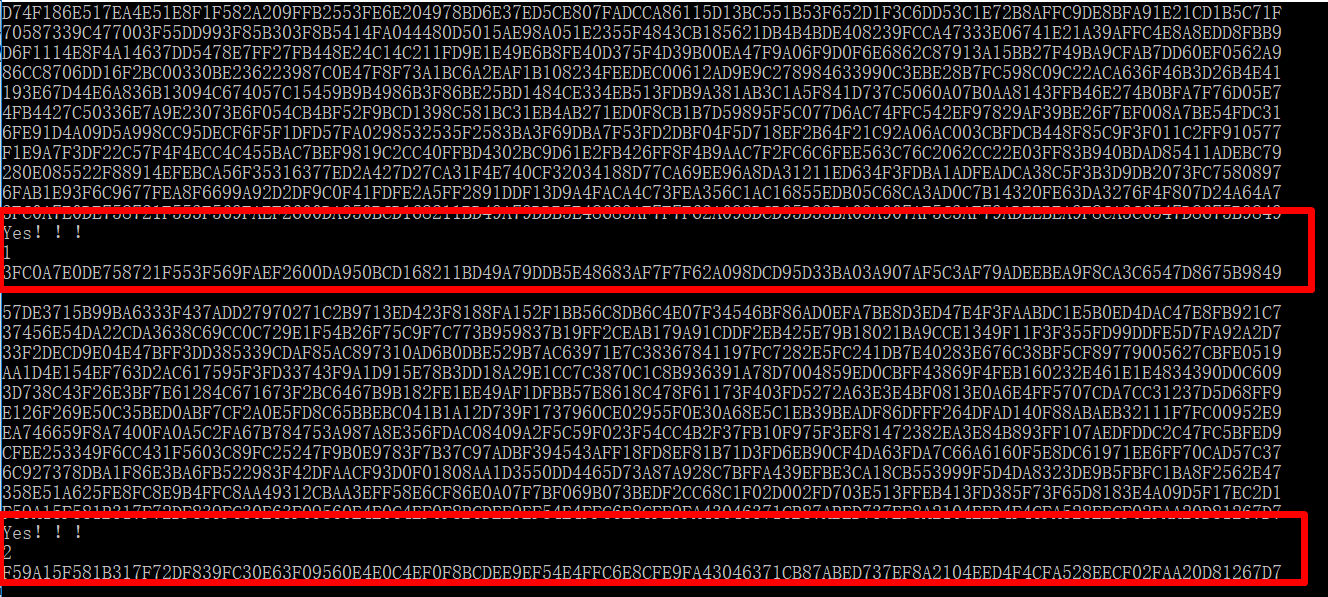
\includegraphics[width=0.78\textwidth]{prime.PNG}
	
	\label{fig:grade}
\end{figure}

生成素数的原理如下:\par 

首先生成512比特的随机数,然后对小于2000的素数取模,若能整除,则重新生成随机数。如果不能整除,则继续对其进行5次Rabin-Miller检测,只要有一次不符合,就可以断定其不是素数,需重新生成素数并重新素性检测,若能够符合,则其有很大可能为素数(概论为96.8\%),将其输出.




程序框图如下:\par 

	\begin{center}
	
	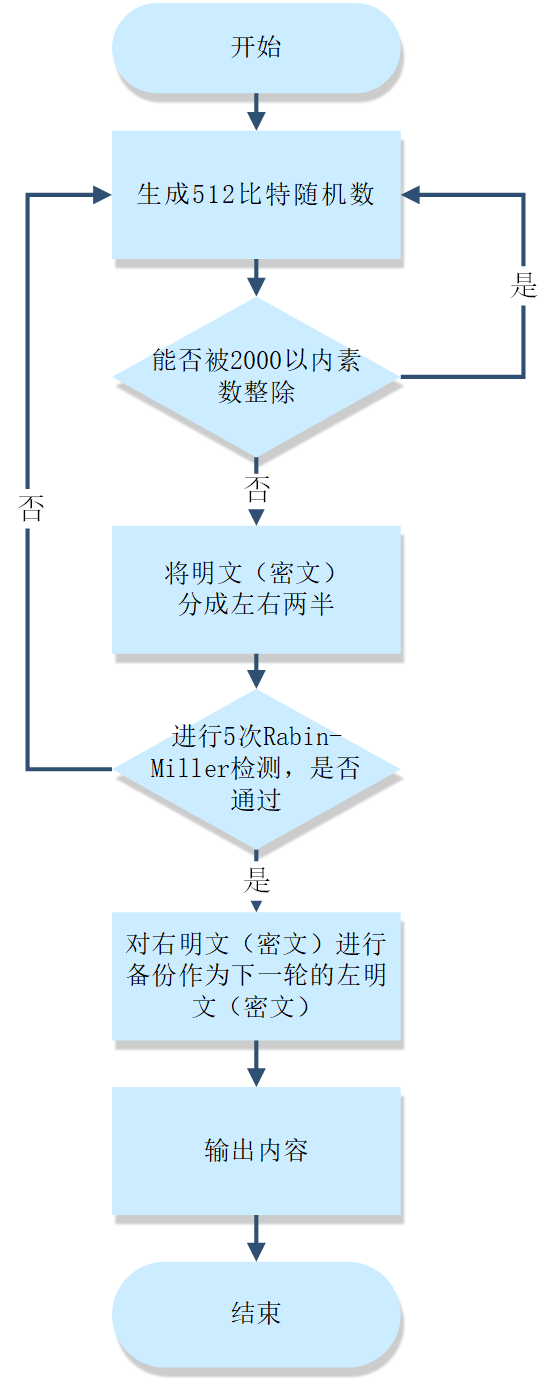
\includegraphics[width=0.28\textwidth]{shengcheng.PNG}

\end{center}


\subsection{RSA加密解密}	
程序框图如下:\par 
	\begin{center}
	
	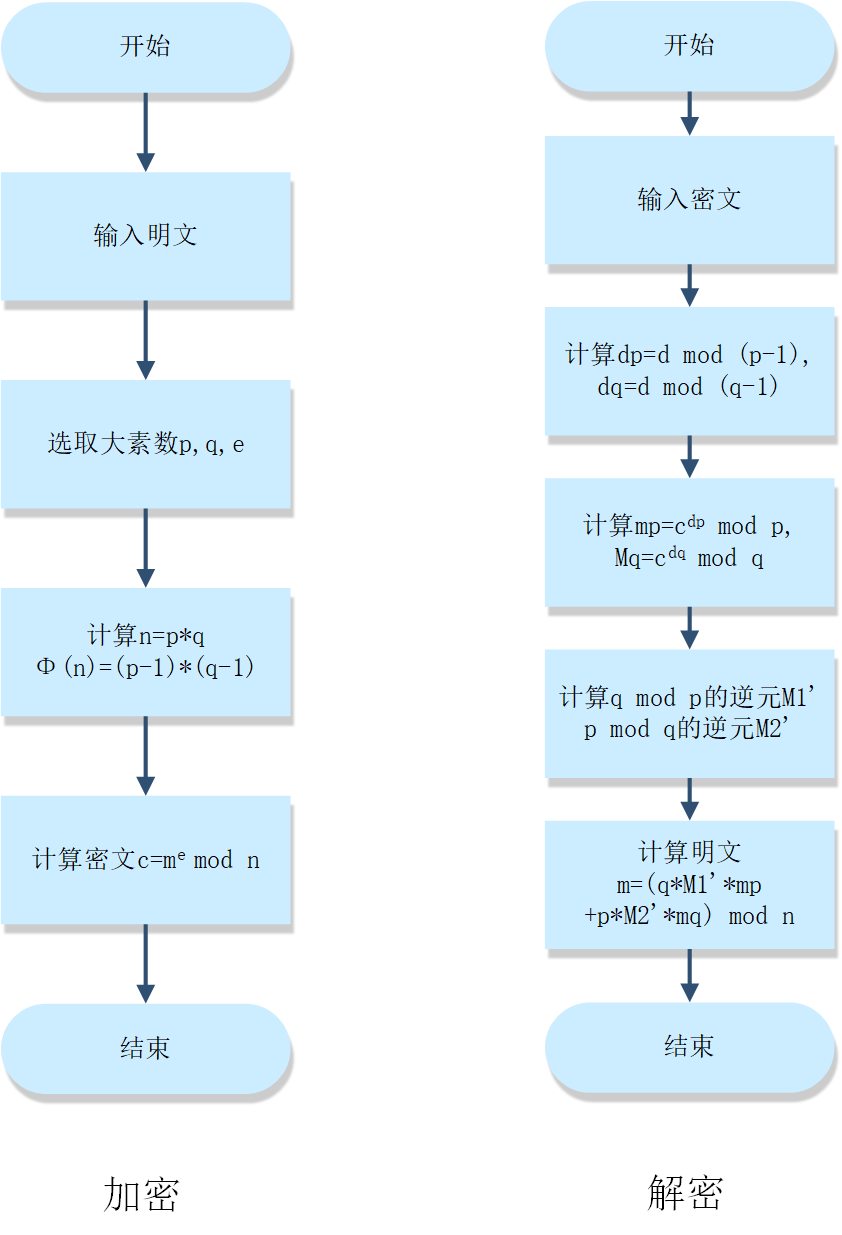
\includegraphics[width=0.3\textwidth]{ende.PNG}
	
\end{center}

代码运行后,进行加密解密结果如下:\par 
	
	\begin{figure}[!ht]
		
		\centering
		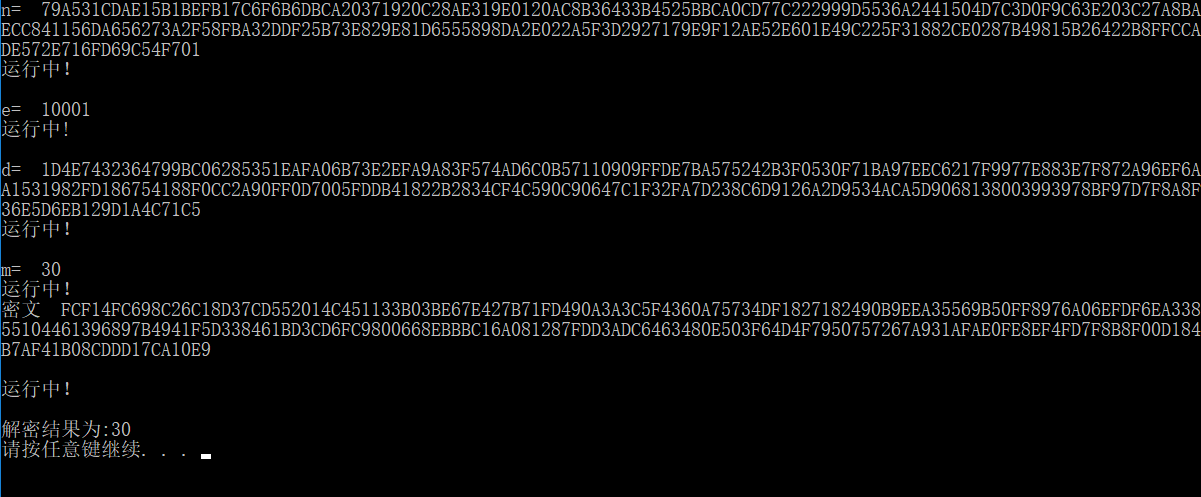
\includegraphics[width=0.8\textwidth]{myen.PNG}
		
		\label{fig:grade}
	\end{figure}


使用RSA-tool进行检验,验证结果是正确的:\par 





\begin{figure}[!ht]
	
	\centering
	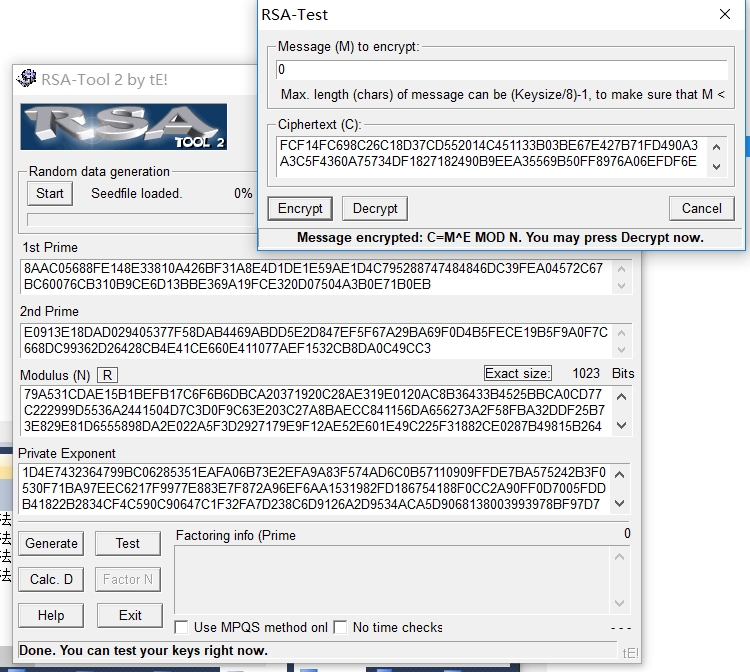
\includegraphics[width=0.8\textwidth]{en.PNG}
	
	\label{fig:grade}
\end{figure}







\begin{figure}[htbp] 
	\begin{minipage}[t]{0.5\linewidth} 
		\centering 
		\includegraphics[width=0.95\textwidth]{1OHPLOTRESPONSE.PNG}
		\caption{fig1} 
		\label{fig:side:a} 
	\end{minipage}% 
	\begin{minipage}[t]{0.5\linewidth} 
		\centering 
		\includegraphics[width=0.95\textwidth]{1OHPLOTRESPONSE.PNG}
		\caption{fig2} 
	\end{minipage} 
\end{figure}  










\end{document}
